\documentclass[12pt]{article}

\usepackage{url}
\usepackage{fullpage}
\usepackage{amssymb,amsfonts}
\usepackage{amsmath}
\newcommand{\eps}{\varepsilon}
\newcommand{\R}{\mathbb{R}}

\usepackage{listings}
\usepackage{color}
\usepackage{graphicx}

\usepackage{varwidth}

\usepackage{hyperref}
\hypersetup{
    linktoc=all,     %set to all if you want both sections and subsections linked
    colorlinks=true,
    linkcolor=blue,
    filecolor=magenta,      
    urlcolor=cyan,
}

\definecolor{dkgreen}{rgb}{0,0.6,0}
\definecolor{gray}{rgb}{0.5,0.5,0.5}
\definecolor{mauve}{rgb}{0.58,0,0.82}

\lstset{frame=tb,
  language=Python,
  aboveskip=3mm,
  belowskip=3mm,
  showstringspaces=false,
  columns=flexible,
  basicstyle={\small\ttfamily},
  numbers=none,
  numberstyle=\tiny\color{gray},
  keywordstyle=\color{blue},
  commentstyle=\color{dkgreen},
  stringstyle=\color{mauve},
  breaklines=true,
  breakatwhitespace=true,
  tabsize=3
}

\usepackage[toc,page]{appendix}

\DeclareMathOperator*{\E}{\mathbb{E}}
\let\Pr\relax
\DeclareMathOperator*{\Pr}{\mathbb{P}}

\DeclareMathOperator*{\Lap}{\text{Lap}}

\DeclareMathOperator*{\Geo}{\text{Geo}}

\def\cl{\lstinline}

\title{CS 208 Homework 2}
\author{Andrew Shackelford}
\date{March 12, 2019}
\setcounter{tocdepth}{3}

\begin{document}

\maketitle

\textbf{All code and figures are available \href{https://github.com/andrew-shackelford/cs208/tree/master/2}{here}}.

{
  \hypersetup{linkcolor=black, hidelinks}
  \tableofcontents
}

\newpage

\section{Problem 1}

\subsection{Part A}

\subsubsection*{Mechanism 1}

\noindent

First, we will examine the mechanism without clamping. This mechanism is clearly $0.5$-DP, since we are adding Laplace noise with scale $\frac{2}{n}$. By the definition of differential privacy, the mechanism is closed under post-processing, that is, for any $\epsilon$-DP mechanism $M$ and any function $f$, $f(M)$ is also $\epsilon$-DP. As a result, applying our clamping function to the $0.5$-DP result will not change how differentially private our release is.

\bigskip

Therefore, this mechanism is $0.5$-DP.

\subsubsection*{Mechanism 2}

Consider the worst-case scenario where $\bar{x} = 0$ yet $\bar{x'} = 1$. In this scenario, it is mathematically impossible for $M(x') < 0$, since the $|Z| \leq 1$. As a result, if $T$ is equal to $\{-0.1\}$, there is no $\epsilon$ such that $\Pr[M(D, q) \in T] \leq e^\epsilon \cdot \Pr[M(D', q) \in T]$, since $\Pr[M(D', q) \in T] = 0$ while $\Pr[M(D, q) \in T]$ is non-zero. As a result, this mechanism is not differentially private for any finite $\epsilon$.

\subsubsection*{Mechanism 3}

\noindent

Consider the definition of $\epsilon$-differential privacy:

$$\Pr[M(D, q) \in T] \leq e^\epsilon \cdot \Pr[M(D', q) \in T]$$
We will consider the worst-case scenario, where $D$ includes one person with value 1 and $D'$ includes one person with value 0. In this case, $M(D)$ will always equal 1, while $M(D')$ will always equal 0. As a result, if $T = \{1\}$, $\Pr[M(D, q) \in T] = 1$ while $\Pr[M(D', q) \in T] = 0$. Therefore, there is no finite $\epsilon$ such that $1 \leq e^\epsilon \cdot 0$, and this mechanism is not differentially private for any finite $\epsilon$.

\subsubsection*{Mechanism 4}

\noindent

We begin by calculating the probability that $M(x)$ is equal to some response $y$:

\begin{align*}
\Pr[M(x) = y] &= \frac{\exp(-n \cdot |y - \bar{x}|/10)}{\int_0^1 \exp(-n \cdot |z-\bar{x}|/10) dz} \\
\end{align*}

Now, we calculate the probability that $M(x')$ is equal to some response $y$:

\begin{align*}
\Pr[M(x') = y] &= \frac{\exp(-n \cdot |y - \bar{x'}|/10)}{\int_0^1 \exp(-n \cdot |z-\bar{x'}|/10) dz} \\
\end{align*}

Dividing one by the other, we find:

\begin{align*}
\frac{\Pr[M(x) = y]}{\Pr[M(x') = y]} &= \frac{\frac{\exp(-n \cdot |y - \bar{x}|/10)}{\int_0^1 \exp(-n \cdot |z-\bar{x}|/10) dz}}{\frac{\exp(-n \cdot |y - \bar{x'}|/10)}{\int_0^1 \exp(-n \cdot |z-\bar{x'}|/10) dz}} \\
&= \frac{\exp(-n \cdot |y - \bar{x}|/10)}{\exp(-n \cdot |y - \bar{x'}|/10)}  \cdot \frac{\int_0^1 \exp(-n \cdot |z-\bar{x}|/10) dz}{\int_0^1 \exp(-n \cdot |z-\bar{x'}|/10) dz} \\
&= \exp(\frac{-n \cdot (|y - \bar{x}| - |y - \bar{x'}|)}{10})  \cdot \int_0^1 \frac{\exp(-n \cdot |z-\bar{x}|/10)}{\exp(-n \cdot |z-\bar{x'}|/10)} dz \\
&\leq \exp(\frac{n \cdot GS_q}{10})  \cdot \int_0^1 \exp(\frac{-n \cdot (|z-\bar{x}| - |z-\bar{x'}|)}{10}) dz \\
&\leq \exp(\frac{n \cdot \frac{1}{n})}{10})  \cdot \int_0^1 \exp(\frac{n \cdot \frac{1}{n}}{10}) dz \\
&\leq \exp(\frac{1}{10})  \cdot \int_0^1 \exp(\frac{1}{10}) dz \\
&\leq \exp(\frac{1}{10})  \cdot \exp(\frac{1}{10}) \\
&\leq \exp(\frac{2}{10}) \\
\end{align*}

Therefore, this mechanism is $0.2$-DP.

\newpage

\subsection{Part B}

\subsubsection*{Mechanism 2}

\noindent

To determine what value of $\delta$ we need, we must consider the global sensitivity of the dataset. Since we are only releasing the mean, the global sensitivity, $GS_q = \frac{1}{n}$. As a result, $Z \sim \Lap(\frac{2}{n})$ means that $\epsilon = 0.5$. However, we now must consider what parts of $Z$ will get clipped by the function and thus not fulfill our $\epsilon = 0.5$.

In order to do so, we must calculate what percentage of our Laplace distribution falls outside of $[-1, 1]$. Integrating the Laplace PDF with mean zero:

\begin{align*}
&1 - \int_{-1}^1 \frac{1}{2s} \exp(-\frac{|y|}{s}) dy \\
&1 - [\int_{-1}^0 \frac{1}{2\frac{2}{n}} \exp(-\frac{-y}{\frac{2}{n}}) dy + \int_0^1 \frac{1}{2\frac{2}{n}} \exp(-\frac{y}{\frac{2}{n}}) dy] \\
&1 - [\frac{1}{2} - \frac{e^{-n/2}}{2} + \frac{1}{2} - \frac{e^{-n/2}}{2}] \\
&1 - [1 - e^{-n/2}] \\
&e^{-n/2} \\
\end{align*}

By the definition of $(\epsilon, \delta)$-DP:

$$\Pr[M(D, q) \in T] \leq e^\epsilon \cdot \Pr[M(D', q) \in T] + \delta$$

we see that we only need consider the part of the tail when $\Pr[M(D', q)] = 0$, and not when $\Pr[M(D, q)] = 0$. 

\medskip

Since our noise distribution is symmetric, we can simply divide our result by half, As a result, our $\epsilon$-DP mechanism fails with probability $\frac{e^{-n/2}}{2}$, so our mechanism is $(0.5, \frac{e^{-n/2}}{2})$-DP.


\subsubsection*{Mechanism 3}

\noindent

As we detailed in part A, we know that it is possible for $M(x) = 1$ with probability 1 if $\bar{x} = 1$, regardless of $n$, and equal 0 with probability 1 if $\bar{x} = 0$. As detailed above, when considering a scenario where $\bar{x} \in \{0, 1\}$, no value of $\epsilon$ is sufficient. As a result, if we were to try to pick an $\epsilon$, $\epsilon$ would have to depend on $\bar{x}$, which would not be differentially private since we would be using the data to construct the mechanism. As a result, we must assume $\epsilon$ is irrelevant in order to account for the cases where $\bar{x} \in \{0, 1\}$. As a result, we'll at least pick $\epsilon = 0$ in order to minimize our $\epsilon$. Using the $(\epsilon, \delta)$ definition of DP:

\begin{align*}
\Pr[M(D, q) \in T] &\leq e^\epsilon \cdot \Pr[M(D', q) \in T] + \delta \\
\bar{x} &\leq e^0 \cdot \bar{x'} + \delta \\
\bar{x} - \bar{x'} &\leq \delta \\
\frac{1}{n} &\leq \delta \\
\end{align*}

We find that $\delta \geq \frac{1}{n}$, so $\delta$ must be at least $\frac{1}{n}$. Therefore, this mechanism is $(0, \frac{1}{n})$-DP. As noted in lecture, this is not very useful, since picking a random person from the dataset and publishing their data is also $(0, \frac{1}{n})$-DP.

\newpage

\subsection{Part C}

\subsubsection*{Mechanism 1}

\noindent

In order to tune this mechanism's privacy parameter $\epsilon$, I would make the following change:

\medskip

$\epsilon$ is only dependent on both the Laplace noise we add. Therefore, to tune $\epsilon$, simply change the amount of Laplace noise we add to $\frac{1}{\epsilon n}$.

In order to have a tunable data domain, we need to figure out how the domain affects $\epsilon$. Changing $a$ and $b$ would change the global sensitivity $GS_q$, which for a mean query is equal to $\frac{b-a}{n}$. Therefore, with a tunable data domain $[a, b]$, we should set $Z \sim \Lap(\frac{b - a}{\epsilon n})$. 

\subsubsection*{Mechanism 2}

\noindent

In order to tune this mechanism's privacy parameters $\epsilon$ and $\delta$, I would make the following changes:

\begin{itemize}
  \item $\epsilon$ is dependent on the Laplace noise that we add to our output. In fact, for some noise $Z \sim \Lap(\frac{\alpha}{n})$, $\epsilon = \frac{1}{\alpha}$, since $GS_q = \frac{1}{n}$.
  \item $\delta$ is dependent on how we clamp the noise $Z$. As we proved in Part 2, $\delta = \frac{1 - \int_{a}^b \frac{1}{2s} \exp(-\frac{|y|}{s}) dy}{2}$, where $a$ and $b$ are the clamping boundaries. As a result, to tune $\delta$, we simply need to adjust $a$ and $b$ to our satisfaction.
\end{itemize}

\bigskip

In order to have tunable data parameters, we need to figure out how those data parameters would affect our $\epsilon$ and $\delta$. Since we are releasing $\bar{x}$, $GS_q$ is dependent on how much any one data point can change the mean. For a dataset $x \in [a, b]^n$, $GS_q = \frac{b - a}{n}$, which, by definition, is how much any one data point can change the mean.

\medskip

We will simply adjust our $\epsilon$ formula to account for the $GS_q$ variable. Since $\epsilon = \frac{n}{\alpha} \cdot GS_q$, now $\epsilon = \frac{b-a}{\alpha}$.

\medskip

Assuming we want to keep the same relative $Z$ range that covers the mean and is clamped from $-\text{abs}(b-a)$ to $\text{abs}(b-a)$, we can simply use our $\delta$ formula from above where $\delta = \frac{1 - \int_{a}^b \frac{1}{2s} \exp(-\frac{|y|}{s}) dy}{2}$.

\subsubsection*{Mechanism 3}

\noindent

As proven above, our value of $\epsilon$ is irrelevant because it depends on $\bar{x}$, which would not be differentially private. To tune $\delta$ requires modifying the global sensitivity of the mechanism, which is dependent on $[a, b]$. Since $\delta = GS_q$, $\delta = \frac{b-a}{n}$, and $b - a = \delta \cdot n$.

\subsubsection*{Mechanism 4}

\noindent

Looking back at our formula and resulting $\epsilon$ for mechanism 4, we find that $\epsilon$ is dependent on the coefficients in the exponential PDF. As a result, for a $M(x) = Y$ where Y has PDF $f_Y$ given by:

$$
f_Y(y) =
\begin{cases}
\frac{\exp(-n \cdot |y - \bar{x}|/\alpha)}{\int_0^1 \exp(-n \cdot |z-\bar{x'}|/\alpha) dz} & \text{if } y \in [0, 1] \\
0 & \text{if } y \not\in [0, 1] \\
\end{cases}
$$

we find that $\epsilon = \frac{2}{\alpha}$. Thus, to tune $\epsilon$, we will simply set $\alpha = \frac{2}{\epsilon}$.

\bigskip

To adjust the data domain, we simply have to adjust the range of the integral as well as the global sensitivity of the query. Using our equations from Part A, we find that:

\begin{align*}
\frac{\Pr[M(x) = y]}{\Pr[M(x') = y]} &\leq \exp(\frac{n \cdot GS_q)}{\alpha})  \cdot \int_a^b \exp(\frac{n \cdot GS_q}{\alpha}) dz \\
&\leq \exp(\frac{n \cdot \frac{b-a}{n})}{\alpha})  \cdot \int_a^b \exp(\frac{n \cdot \frac{b-a}{n}}{\alpha}) dz \\
&\leq \exp(\frac{b-a}{\alpha})  \cdot \int_a^b \exp(\frac{b-a}{\alpha}) dz \\
&\leq \exp(\frac{b-a}{\alpha})  \cdot (b-a) \cdot \exp(\frac{b-a}{\alpha}) \\
&\leq (b-a) \cdot \exp(\frac{2 \cdot (b-a)}{\alpha}) \\
&\leq \exp(\frac{2 \cdot (b-a) + \ln (b-a)}{\alpha}) \\
\end{align*}

Solving for $\alpha'$, we find:

\begin{align*}
\epsilon &= \frac{2 \cdot (b-a) + \ln (b-a)}{\alpha'} \\
\alpha' &= \frac{2 \cdot (b-a) + \ln (b-a)}{\epsilon} \\
\end{align*}

Therefore, with tunable parameter $\epsilon$ and data domain $[a, b]$, we should set $M(x) = Y$ where $Y$ has PDF $f_Y$ given by:

$$
f_Y(y) =
\begin{cases}
\frac{\exp(-n \cdot |y - \bar{x}|/\alpha)}{\int_a^b \exp(-n \cdot |z-\bar{x'}|/\alpha) dz} & \text{if } y \in [a, b] \\
0 & \text{if } y \not\in [a, b] \\
\end{cases}
$$

where $\alpha = \frac{2 \cdot (b-a) + \ln (b-a)}{\epsilon}$.

\newpage

\subsection{Part D}

\noindent

I consider Mechanism 1 to be the best for releasing a mean for the following reasons:

\begin{itemize}
    \item Firstly, this mechanism is $\epsilon$-DP with no $\delta$. As such, it always meets its differentially private guarantee.
    \item Secondly, this mechanism ensures every mean falls within the domain $[a, b]$, thus satisfying the traditional definition of a mean. While data scientists would understand how differentially private releases might fall outside the domain, this makes the data easier to interpret for everyone, and fall within guidelines for certain organizations like the Census Bureau.
    \item Lastly, this mechanism is simple -- it is simply a mean, plus noise, clamped to the data domain. The result is clamped rather than the noise, which is easier to understand and will keep the values within the domain, it releases a much more precise value than Mechanism 3 which either releases 1 or 0, and is vastly simpler than Mechanism 4, which requires calculating and normalizing a PDF for each $\bar{x}$.
\end{itemize}

\newpage

\section{Problem 2}

\subsection{Part A}

\noindent

See the \cl{poisson_dataset()} function in \cl{problem_2.py}, available at Appendix \ref{appendix:problem_2}.

\subsection{Part B}

\noindent

I chose to implement Mechanism 2. See the \cl{mech_2_release()} function in \cl{problem_2.py}, available at Appendix \ref{appendix:problem_2}.

\subsection{Part C}

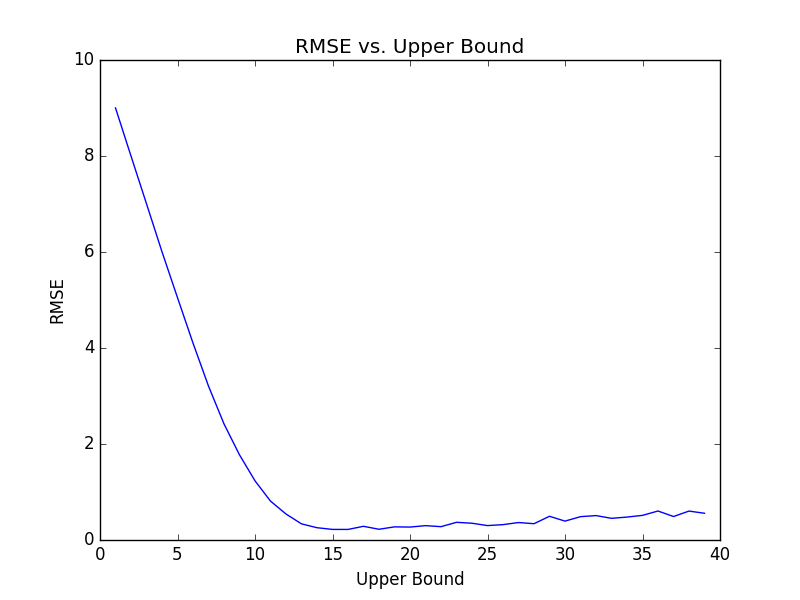
\includegraphics[scale=0.6]{problem_2.png}

Looking at the results, it seems that the approximate optimal value $b^* = 15$.

\subsection{Part D}

\noindent

This approach is not safe because we are still essentially using our non-private dataset to determine $b^*$. Even though we are bootstrapping, we are still sampling from our non-private dataset $x$ and thus our bootstrapped dataset $x'$ still contains information about $x$.

\medskip

Suppose there is some outlier member $a \in x$. When constructing a nonparametric bootstrap $x'$ of size $n$, the probability that any random member $a$ is not in $x'$ is equal to $(\frac{n-1}{n})^n$. $\lim_{n \to \infty} (\frac{n-1}{n})^n = \frac{1}{e}$, so the probability that $a \in x'$ for any moderately large $n$ is approximately $1 - \frac{1}{e} \approx 0.63$. As a result, there is a significant probability that $a \in x'$ and thus would change $b^*$ - a change that would not occur if $a$ were not in $x$. As a result, using values from our bootstrapped dataset $x'$ to calculate $b^*$ necessarily violates differential privacy, since with high probability $b^*$ would be changed by the inclusion of a single row in the dataset.

\subsection{Part E}

\noindent

An alternative method to calculating $b^*$ in a differentially private manner would be to use a similar public dataset, or use some priors we already had before looking at our private dataset. For example, if releasing statistics about Harvard College students, we could clip the age of students to 25, just based on our common knowledge of the age of graduating college students in the United States. Similarly, we could try to find a similar public dataset of Yale students and calculate our upper bound using those statistics.

\newpage

\section{Problem 3}

\subsection{Part A}

\noindent

I chose to clamp the $x_i$'s using the values I determined in Problem 2, that is $[0, 15]$. I then chose to clamp the $y_i$'s to $[-5, 20]$ to allow for the addition of $\alpha$ as well as noise from the normal distribution. In this case, almost all the $y_i$'s should not be clamped any more than the $x_i$'s, since $\alpha = 1$ and the standard deviation of the noise $\sigma = 1$. The code for this differentially-private release is located in the \cl{regression_release()} function of \cl{problem_3.py}, located at Appendix \ref{appendix:problem_3}.

\subsection{Part B}

The code for this plot is located in the \cl{part_b()} function of \cl{problem_3.py}, located at Appendix \ref{appendix:problem_3}.

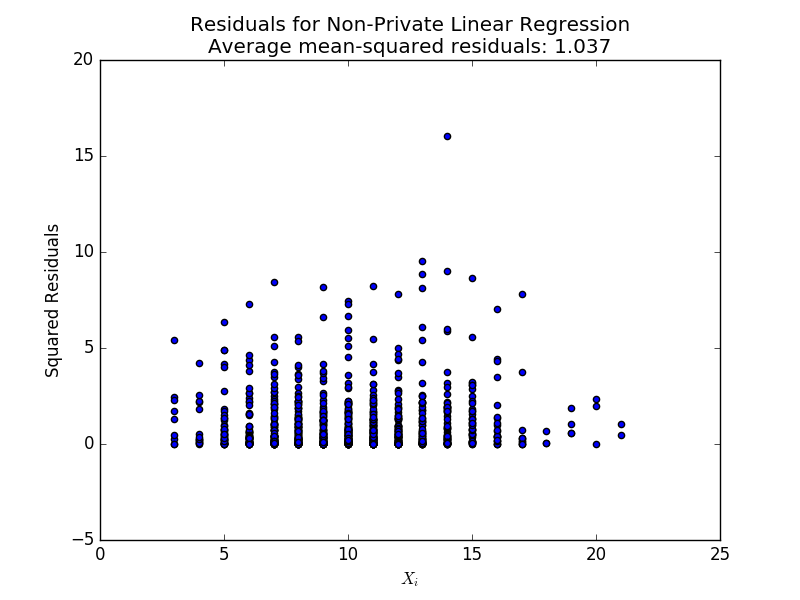
\includegraphics[scale=0.4]{problem_3_non_private.png} 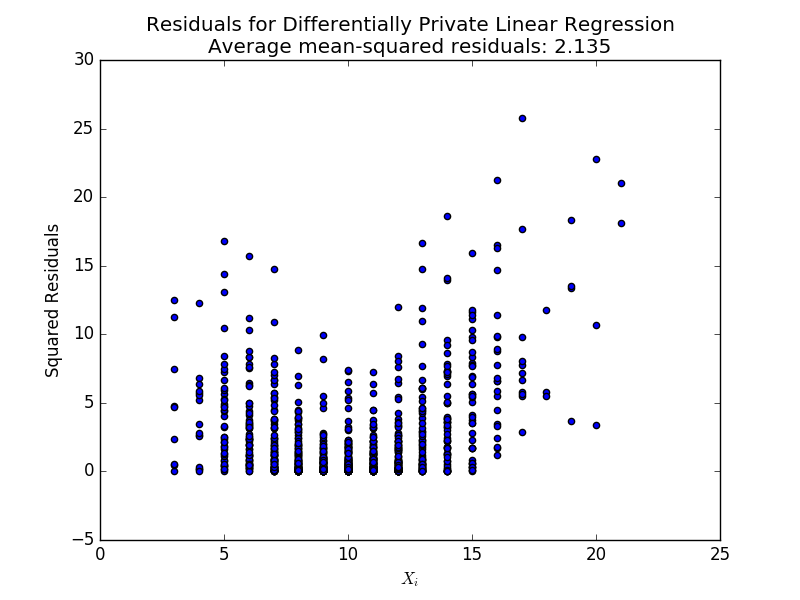
\includegraphics[scale=0.4]{problem_3_differentially_private.png}

As we can see in the above plot, the non-private algorithm has better utility 1.037 (where lower mean-squared residuals indicates better utility) than the differentially private algorithm's utility of 2.135. However, the differentially private release only reduces utility by approximately 2x, which is still quite good given that the first release lacks any privacy protections at all while the differentially private release is $1$-DP.

\subsection{Part C}

\noindent

Running grid search over various different grids (using a softmax function to ensure all the $\epsilon$'s summed to 1), I found that the best epsilon partition is approximately $[0.4, 0.4, 0.05, 0.15]$, where $\epsilon_{xx} = 0.4$, $\epsilon_{xy} = 0.4$, $\epsilon_{x\_mean} = 0.05$, and $\epsilon_{y\_mean} = 0.15$. The code to perform this grid search is located in the \cl{part_c()} function of \cl{problem_3.py}, located at Appendix \ref{appendix:problem_3}. Below is a results table of all the options tried \textit{(Note: values may not sum to 1 due to rounding)}:

\begin{center}
\begin{tabular}{|c|c|c|c|c|}
\hline
 $\epsilon_{xx}$ & $\epsilon_{xy}$ & $\epsilon_{x\_mean}$ & $\epsilon_{y\_mean}$ & Mean-squared residuals \\ \hline
0.4 & 0.4 & 0.05 & 0.15&1.601\\ \hline
0.37 & 0.37 & 0.13 & 0.13&1.713\\ \hline
0.4 & 0.4 & 0.15 & 0.05&1.908\\ \hline
0.64 & 0.24 & 0.03 & 0.09&2.012\\ \hline
0.25 & 0.25 & 0.25 & 0.25&2.186\\ \hline
0.24 & 0.64 & 0.03 & 0.09&2.477\\ \hline
0.17 & 0.48 & 0.17 & 0.17&2.678\\ \hline
0.24 & 0.64 & 0.09 & 0.03&3.001\\ \hline
0.64 & 0.24 & 0.09 & 0.03&3.108\\ \hline
0.17 & 0.17 & 0.17 & 0.48&3.502\\ \hline
0.17 & 0.17 & 0.48 & 0.17&3.711\\ \hline
0.48 & 0.17 & 0.17 & 0.17&3.719\\ \hline
0.09 & 0.24 & 0.64 & 0.03&7.006\\ \hline
0.09 & 0.64 & 0.03 & 0.24&7.598\\ \hline
0.09 & 0.24 & 0.03 & 0.64&7.774\\ \hline
0.09 & 0.64 & 0.24 & 0.03&8.577\\ \hline
0.64 & 0.09 & 0.24 & 0.03&14.136\\ \hline
0.08 & 0.08 & 0.22 & 0.61&14.958\\ \hline
0.13 & 0.13 & 0.37 & 0.37&21.25\\ \hline
0.24 & 0.09 & 0.64 & 0.03&23.799\\ \hline
0.08 & 0.08 & 0.61 & 0.22&24.571\\ \hline
0.03 & 0.64 & 0.24 & 0.09&36.405\\ \hline
0.03 & 0.24 & 0.09 & 0.64&38.393\\ \hline
0.03 & 0.24 & 0.64 & 0.09&40.352\\ \hline
0.03 & 0.64 & 0.09 & 0.24&40.691\\ \hline
0.03 & 0.09 & 0.64 & 0.24&53.327\\ \hline
0.03 & 0.09 & 0.24 & 0.64&54.066\\ \hline
0.24 & 0.09 & 0.03 & 0.64&136.785\\ \hline
0.09 & 0.03 & 0.64 & 0.24&175.423\\ \hline
0.24 & 0.03 & 0.64 & 0.09&281.167\\ \hline
0.64 & 0.03 & 0.24 & 0.09&294.29\\ \hline
0.24 & 0.03 & 0.09 & 0.64&862.15\\ \hline
0.09 & 0.03 & 0.24 & 0.64&1207.091\\ \hline
0.64 & 0.03 & 0.09 & 0.24&4231.524\\ \hline
0.64 & 0.09 & 0.03 & 0.24&4329.301\\ \hline
\end{tabular}
\end{center}

Looking at these results, it appears that keeping the $\epsilon$'s for $xx$ and $xy$ high is more important than the $\epsilon$'s for the means. This makes sense because the $xx$ and $xy$ are used to calculate the $\beta$ coefficient for the linear regression which, if wrong, could wildly change the shape of the graph, whereas the means are simply used to calculate the $\alpha$ for the $y$-intercept, which would just shift the graph slightly. Using the \cl{part_c_optimized()} function of \cl{problem_3.py}, located at Appendix \ref{appendix:problem_3}, to test a further optimized $\epsilon$ partition of $[0.4, 0.4, 0.1, 0.1]$, we obtain a mean squared residual of $1.552$, considerably better than the equal partition's result of $2.135$. This further confirms our hypothesis that the $xx$ and $xy$ $\epsilon$'s matter much more than the $x_{mean}$ and $y_{mean}$ $\epsilon$'s.

\newpage

\section{Problem 4}

We seek to prove that:

\begin{align*}
\E[\#\{i \in [n]: A(M(x))_i = X_i\}/n] &\leq e^\epsilon \cdot \max\{p, 1-p\} + \delta \\
\end{align*}

Let $I_i$ be an indicator variable representing the event that the adversary correctly guesses $X_i$, that is $I_i = A(M(x))_i = X_i$. Substituting the indicator variable back in, we find:

\begin{align*}
\E[\#\{i \in [n]: I_i/n] &\leq e^\epsilon \cdot \max\{p, 1-p\} + \delta \\
\sum_{i=1}^N \E[I_i/n] &\leq e^\epsilon \cdot \max\{p, 1-p\} + \delta \\
\frac{1}{n} \sum_{i=1}^N \E[I_i] &\leq e^\epsilon \cdot \max\{p, 1-p\} + \delta \\
\end{align*}

Using symmetry and the fundamental bridge between probability and expectation:
\begin{align*}
\frac{1}{n} \sum_{i=1}^N \Pr[I_i] &\leq e^\epsilon \cdot \max\{p, 1-p\} + \delta \\
\Pr[I] &\leq e^\epsilon \cdot \max\{p, 1-p\} + \delta \\
\end{align*}

where $I$ is the indicator variable for any random $x$ in the dataset. Now, consider a query as to whether $x$ has the sensitive bit set to 1, and that same query against a different random row in the dataset. By the definition of differential privacy:

$$\Pr[M(D, q) \in T] \leq e^\epsilon \cdot \Pr[M(D', q) \in T] + \delta$$

Since $\Pr[M(D', q) \in T]$ is equal to the probability that a random row in the dataset has the sensitive bit set to 1, $\Pr[M(D', q) \in T] = p$. As a result,

$$\Pr[M(D, q) \in T] \leq e^\epsilon \cdot p + \delta$$

\bigskip

By symmetry, the same analysis applies to see if $x$ has the sensitive bit set to 0, so $$\Pr[M(D, q) \in T] \leq e^\epsilon \cdot (1-p) + \delta$$

Therefore, $\Pr[M(D, q) \in T] \leq e^\epsilon \cdot \max\{p, 1-p\} + \delta$, where $\Pr[M(D, q) \in T]$ is the probability that a query truthfully reports the sensitive bit of $x$. Since $\Pr[I] = \Pr[M(D, q) \in T]$:

\begin{align*}
\Pr[M(D, q) \in T] &\leq e^\epsilon \cdot \max\{p, 1-p\} + \delta \\
\Pr[I] &\leq e^\epsilon \cdot \max\{p, 1-p\} + \delta \\
\E[\#\{i \in [n]: A(M(x))_i = X_i\}/n] &\leq e^\epsilon \cdot \max\{p, 1-p\} + \delta \\
\end{align*}

As a result, we have proved that the expected fraction of bits that the adversary successfully reconstructs is not much larger than the trivial bound of $\max\{p, 1-p\}$.

\newpage

\begin{appendices}

\section{\cl{problem_2.py}}
\label{appendix:problem_2}

\begin{lstlisting}
"""
Andrew Shackelford
ashackelford@college.harvard.edu

CS 208 - Spring 2019
Homework 2, Problem 2
"""

import numpy as np
import matplotlib.pyplot as plt

# return a poisson dataset of size n with labmda = 10
def poisson_dataset(n):
    return np.random.poisson(lam=10, size=n)

# release the mean of x according to mechanism 2
def mech_2_release(x, epsilon, a, b):
    x = np.clip(x, a, b)
    n = x.shape[0]
    gs_q = (float(b) - float(a)) / float(n)
    s = gs_q / float(epsilon)
    z = np.random.laplace(scale=s)

    mean = np.mean(x)
    z_clamped = np.clip(z, -abs(b-a), abs(b-a))

    return mean + z_clamped

def main():
    # create dataset, variables
    data = poisson_dataset(200)
    a = 0
    epsilon = 0.5
    num_trials = 100
    true_result = np.mean(data)

    # test different upper bounds of b
    x, y = [], []
    for b in range(1, 40):
        se = []
        for i in range(num_trials):
            noisy_result = mech_2_release(data, epsilon, a, b)
            se.append(np.square(noisy_result - true_result))
        rmse = np.sqrt(np.mean(se))
        x.append(b)
        y.append(rmse)

    # plot results
    plt.plot(x, y)
    plt.title('RMSE vs. Upper Bound')
    plt.xlabel('Upper Bound')
    plt.ylabel('RMSE')
    plt.savefig('problem_2.png')

if __name__ == "__main__":
    main()
\end{lstlisting}

\newpage

\section{\cl{problem_3.py}}
\label{appendix:problem_3}

\begin{lstlisting}
"""
Andrew Shackelford
ashackelford@college.harvard.edu

CS 208 - Spring 2019
Homework 2, Problem 3
"""

import numpy as np
import matplotlib.pyplot as plt

def poisson_dataset(n):
    return np.random.poisson(lam=10, size=n)

def regression_release(x, y, epsilon_partitions, x_a, x_b, y_a, y_b):
    # create and clip variables
    n = x.shape[0]
    x = np.clip(x, x_a, x_b)
    y = np.clip(y, y_a, y_b)
    x_mean = np.mean(x)
    y_mean = np.mean(y)
    xx, xy = [], []

    # calculate estimators
    for i in range(n):
        xy.append((x[i] - x_mean) * (y[i] - y_mean))
        xx.append(np.square(x[i] - x_mean))
    xx = np.sum(xx)
    xy = np.sum(xy)

    # calculate scales for xy and xx
    xy_scale = float((x_b-x_a) * (y_b-y_a)) / float(epsilon_partitions[0])
    xx_scale = float(np.square(x_b - x_a)) / float(epsilon_partitions[1])

    # calculate beta and noisy_beta
    beta = float(xy) / float(xx)
    noisy_xy = float(xy) + np.random.laplace(scale=xy_scale)
    noisy_xx = float(xx) + np.random.laplace(scale=xx_scale)
    noisy_beta = noisy_xy / noisy_xx

    # calculate scales for x_mean and y_mean
    x_mean_scale = float(x_b - x_a) / float(n) / float(epsilon_partitions[2])
    y_mean_scale = float(y_b - y_a) / float(n) / float(epsilon_partitions[3])

    # calculate alpha and noisy alpha
    alpha = y_mean - (beta * x_mean)
    noisy_x_mean = float(x_mean) + np.random.laplace(scale=x_mean_scale)
    noisy_y_mean = float(y_mean) + np.random.laplace(scale=y_mean_scale)
    noisy_alpha = noisy_y_mean - (noisy_beta * noisy_x_mean)

    return alpha, beta, noisy_alpha, noisy_beta

# return the value of the linear function
def linear_function(x_i, alpha=1., beta=1., sigma=1.):
    return float(beta) * float(x_i) + float(alpha) + np.random.normal(scale=sigma)

def monte_carlo(epsilon_partitions):
    # create variables
    x_a = 0
    x_b = 15
    y_a = -5
    y_b = 20
    sigma = 1
    n = 1000

    # create datasets and calculate regression
    X = poisson_dataset(n)
    Y = []
    for x_i in X:
        Y.append(linear_function(x_i))
    alpha, beta, noisy_alpha, noisy_beta = regression_release(X, Y, epsilon_partitions, x_a, x_b, y_a, y_b)

    # calculate residuals
    resid_x, resid_y = [], []
    noisy_resid_x, noisy_resid_y = [], []
    for i, x_i in enumerate(X):
        resid_y_i = np.square(Y[i] - beta * x_i - alpha)
        noisy_resid_y_i = np.square(Y[i] - noisy_beta * x_i - noisy_alpha)
        
        resid_x.append(x_i)
        resid_y.append(resid_y_i)
        noisy_resid_x.append(x_i)
        noisy_resid_y.append(noisy_resid_y_i)

    # calculate residual means
    resid = np.mean(resid_y)
    noisy_resid = np.mean(noisy_resid_y)

    return resid_x, resid_y, resid, noisy_resid_x, noisy_resid_y, noisy_resid

def part_b():
    # create variables
    epsilon_partitions = [0.25, 0.25, 0.25, 0.25]
    num_trials = 100

    # get residual plot
    resid_x, resid_y, _, noisy_resid_x, noisy_resid_y, _ = monte_carlo(epsilon_partitions)

    # get averages of mean-squared residuals
    resid_lst = []
    noisy_resid_lst = []
    for _ in range(num_trials):
        _, _, resid, _, _, noisy_resid = monte_carlo(epsilon_partitions)
        resid_lst.append(resid)
        noisy_resid_lst.append(noisy_resid)
    resid = np.mean(resid_lst)
    noisy_resid = np.mean(noisy_resid_lst)

    # plot non-private results
    plt.scatter(resid_x, resid_y)
    plt.title('Residuals for Non-Private Linear Regression\n' +
              'Average mean-squared residuals: ' +
              str(round(resid, 3)))
    plt.xlabel(r'$X_i$')
    plt.ylabel('Squared Residuals')
    plt.savefig('problem_3_non_private.png')
    plt.clf()

    # plot private results
    plt.scatter(noisy_resid_x, noisy_resid_y)
    plt.title('Residuals for Differentially Private Linear Regression\n' +
              'Average mean-squared residuals: ' +
              str(round(noisy_resid, 3)))
    plt.xlabel(r'$X_i$')
    plt.ylabel('Squared Residuals')
    plt.savefig('problem_3_differentially_private.png')
    plt.clf()

# normalize epsilon partitions to sum to 1
def softmax(x):
    return np.exp(x) / np.sum(np.exp(x))

def part_c():
    # create variables and grid
    results = {}
    num_trials = 100
    grids = [
                [1, 1, 1, 1],

                [2, 1, 1, 1],
                [1, 2, 1, 1],
                [1, 1, 2, 1],
                [1, 1, 1, 2],

                [2, 2, 1, 1],
                [3, 3, 2, 1],
                [3, 3, 1, 2],

                [1, 1, 2, 2],
                [1, 1, 2, 3],
                [1, 1, 3, 2],

                [1, 2, 3, 4],
                [1, 2, 4, 3],
                [1, 3, 2, 4],
                [1, 3, 4, 2],
                [1, 4, 2, 3],
                [1, 4, 3, 2],

                [2, 1, 3, 4],
                [2, 1, 4, 3],
                [2, 3, 1, 4],
                [2, 3, 4, 1],
                [2, 4, 1, 3],
                [2, 4, 3, 1],

                [3, 1, 2, 4],
                [3, 1, 4, 2],
                [3, 2, 1, 4],
                [3, 2, 4, 1],
                [3, 4, 1, 2],
                [3, 4, 2, 1],

                [4, 1, 2, 3],
                [4, 1, 3, 2],
                [4, 2, 1, 3],
                [4, 2, 3, 1],
                [4, 3, 1, 2],
                [4, 3, 2, 1],
            ]

    # run grid search
    for epsilon_partitions in grids:
        epsilon_partitions = softmax(epsilon_partitions)
        noisy_resids = []
        for _ in range(num_trials):
            noisy_resids.append(monte_carlo(epsilon_partitions)[-1])
        results[np.mean(noisy_resids)] = epsilon_partitions
        

    # print out latex formatted results table
    print("Results table:")
    for key in sorted(results.keys()):
        ep_1 = round(results[key][0], 2)
        ep_2 = round(results[key][1], 2)
        ep_3 = round(results[key][2], 2)
        ep_4 = round(results[key][3], 2)
        resid = round(key, 3)
        print(str(ep_1) + ' & ' + str(ep_2) + ' & ' + str(ep_3) + ' & ' + str(ep_4) + '&' + str(resid) + '\\\\ \\hline')

    # print out best partition
    print ("best epsilon partition is " +
          str(results[sorted(results.keys())[0]]) +
          " with residuals " +
          str(sorted(results.keys())[0]))

def part_c_optimized():
    # create variables
    epsilon_partitions = [0.40, 0.40, 0.1, 0.1]
    num_trials = 100

    # get averages of mean-squared residuals
    noisy_resid_lst = []
    for _ in range(num_trials):
        _, _, _, _, _, noisy_resid = monte_carlo(epsilon_partitions)
        noisy_resid_lst.append(noisy_resid)
    noisy_resid = np.mean(noisy_resid_lst)

    # print result
    print("mean squared residuals for " +
          str(epsilon_partitions) +
          " is " +
          str(noisy_resid))

def main():
    part_b()
    part_c()
    part_c_optimized()

if __name__ == "__main__":
    main()
\end{lstlisting}

\end{appendices}

\end{document}